\documentclass[12pt]{article}

% --- Page layout ---
\usepackage[margin=1in]{geometry}
\usepackage{setspace}
\doublespacing

% --- Typography and math ---
\usepackage{amsmath, amssymb}
\usepackage[T1]{fontenc}
\usepackage{microtype}

% --- Tables and figures ---
\usepackage{booktabs}
\usepackage{threeparttable}
\usepackage{graphicx}
\usepackage{float}
\usepackage[labelfont=bf]{caption}
\usepackage{dcolumn}

% --- Citations ---
\usepackage[round]{natbib}
\bibliographystyle{plainnat}

% --- Hyperlinks ---
\usepackage[colorlinks=true, citecolor=black, linkcolor=black, urlcolor=black]{hyperref}

% --- Section formatting ---
\usepackage{titlesec}
\titleformat{\section}{\large\bfseries}{\thesection}{1em}{}
\titleformat{\subsection}{\normalsize\bfseries}{\thesubsection}{1em}{}

% ==========================================================================
\begin{document}

\title{Data Center Alley:
       Tax Incidence, Property Values, and the Political Economy
       of Infrastructure Siting in Loudoun County, Virginia}

\author{Christopher Nesseth}

\maketitle
\thispagestyle{empty}

\vfill

\begin{abstract}
\singlespacing
\noindent In March 2025, Loudoun County, Virginia eliminated by-right data center development, shifting approvals to Special Exception review. I assess whether the cost-benefit incidence justifies this relocation of approval rights or whether the shift reflects NIMBY capture by a concentrated minority. Tax revenue from the county's roughly 200 data centers funds a residential rate cut worth about \$2,512 per year to all 130,000 county homeowners. Data-center-driven grid costs of \$168--\$444 per residential customer per year fall on 2.36 million Dominion ratepayers statewide, who have no standing in Loudoun's permit process. A \citet{SunAbraham2021} cohort-robust event study on 31,333 resale transactions (2020--2025) yields an ATT of $-1.3$ percent ($p < 0.01$) that is specification-sensitive and does not robustly identify harm at any single radius. The benefit is large and broadly shared. The harm is concentrated, fragile, and economically modest. The incidence pattern fits more closely with NIMBY capture of decision rights than with a welfare-justified reallocation of approval authority.
\end{abstract}

\newpage
\setcounter{page}{1}


% ==========================================================================
\section{Introduction}
\label{sec:intro}
% ==========================================================================

Loudoun County, Virginia is the largest data center market in the world. Its roughly 200 data center facilities generate an estimated \$895 million in annual tax revenue (about one-third of the county's entire operating budget) and have enabled the Board of Supervisors to reduce the residential real property tax rate every year for more than a decade, from \$1.145 per \$100 of assessed value in 2012 to \$0.805 in 2025. At the current median assessed value of \$738,730, this rate reduction saves the typical homeowner about \$2,512 per year. Loudoun's residential tax rate is now 28~percent below Fairfax County's (\$1.125) and 13~percent below Prince William County's (\$0.920), a gap likely reflecting in large part data center revenue. Yet on March 18, 2025, the Board of Supervisors voted to eliminate by-right data center development across the county, requiring each new facility to obtain a Special Exception through public hearings. Does the incidence pattern justify this relocation of approval rights, or does the shift reflect NIMBY capture of decision rights by a concentrated minority?

This paper investigates the distributional incidence of data center development through three channels. The first channel is fiscal. I combine the county's annual residential tax rate history with current assessed-value data to estimate the per-household share of data-center-funded rate relief, and benchmark Loudoun's rate against neighboring jurisdictions that lack a comparable data center tax base. The second channel is electricity rates. I allocate the data-center-driven transmission and distribution capital expenditure documented by \citet{JLARC2024} across residential customers in Dominion Energy Virginia's service territory. The third channel is property values. I assemble a panel of 31,333 residential resale transactions from 2020 to 2025 and exploit staggered data center permit dates across roughly 130 facilities as treatment events in a hedonic difference-in-differences (DiD) design. The primary specification is the \citet{SunAbraham2021} cohort-robust interaction-weighted estimator, with parallel-trends diagnostics, a leave-one-tract-out jackknife, a placebo permutation test, and a continuous cumulative-exposure measure that exploits time-varying treatment intensity rather than arbitrary distance cutoffs.

The weight of the evidence reveals a substantial asymmetry with large fiscal benefits that accrue to all county homeowners. Electricity costs are real but diffuse, borne statewide, and being addressed through rate design reform. The hedonic design does not find robust evidence of economically meaningful property value harm, and the cumulative exposure specification is radius-sensitive (null at 2~km, modestly negative at 4~km) rather than cleanly identified at any single radius. This incidence pattern (large diffuse benefits alongside weak evidence of localized harm) complicates a straightforward welfare justification for the 2025 reallocation of approval rights. The institutional arrangement separated who captured fiscal gains, who bore localized burdens, and who held approval authority. Whether the incidence pattern justifies that reallocation of decision rights, or whether the shift instead reflects NIMBY capture by a concentrated minority, is the question this paper tries to answer.

The paper contributes to several literatures. It provides the first quasi-experimental estimate of data center proximity effects on residential property values, extending the infrastructure disamenity literature on power plants \citep{Davis2011}, toxic facilities \citep{Currie2015}, shale gas \citep{Muehlenbachs2015}, and wind turbines \citep{Gibbons2015, Jarvis2025}. It contributes to the fiscal impact literature \citep{Greenstone2010, Bartik2020, Slattery2020} by documenting the unusually large tax base contribution of data centers under Virginia's Business Personal Property (BPP) structure. And it connects the empirical evidence to the political economy of "not in my backyard" (NIMBY) opposition and infrastructure siting, building on \citet{Olson1965}, \citet{Fischel2001}, and \citet{GlaeserGyourko2018}.

% ==========================================================================
\section{Background}
\label{sec:background}
% ==========================================================================

The Ashburn corridor of Loudoun County, Virginia is the largest data center (DC) market in the world. The concentration traces to a single infrastructure decision. In 1992, the Metropolitan Area Ethernet exchange point MAE-East was established near Dulles International Airport, making Ashburn one of only four original internet exchange nodes in the United States. The low-latency advantage of co-location near this exchange attracted the first wave of internet companies in the mid-1990s. When the dot-com bubble burst in 2001, many facilities stood vacant, but the underlying fiber infrastructure remained, and the corridor proved durable. Recovery was gradual through the 2000s and then accelerated sharply as cloud computing scaled.

By the early 2010s, Ashburn had earned the informal designation "Data Center Alley.'' Today Loudoun County is home to roughly 200 data centers (more than any other jurisdiction on earth), and the county's permit records show roughly 49 million square feet of data center space permitted across about 130 parcels by early 2026, up from 29 million square feet in 2020 \citep{LoudounCOR2025}. Northern Virginia as a whole had surpassed 4,900 megawatts (MW) of operational data center capacity by Q1 2025, with Loudoun County accounting for roughly half of the state's data centers by number of sites, square footage, and energy usage \citep{JLARC2024}. Hyperscale facilities (those operated by Amazon Web Services, Microsoft Azure, Google Cloud, and Meta) held about 53 percent of the Northern Virginia market share in 2025 \citep{JLARC2024}.

The fiscal transformation of Loudoun County is striking. The county levies a BPP tax on the computer equipment and servers housed in data centers. Because this equipment depreciates rapidly and turns over frequently, it generates large and growing annual assessments. Data center tax revenues grew roughly six-fold over the past decade, from about \$146 million in FY2016 to an estimated \$895 million in FY2025, with the county's adopted budget projecting continued growth toward \$1.3 billion by FY2027 \citep{JLARC2024, LoudounFinance2024}. JLARC estimated that data centers contribute \$9.1 billion to Virginia GDP and support 74,000 jobs statewide annually \citep{JLARC2024}.

This revenue has allowed the Board of Supervisors to reduce the residential real property tax rate every year for more than a decade, from \$1.145 per \$100 assessed value in tax year 2012 to \$0.805 in 2025 \citep{LoudounCOR2025}. The resulting tax advantage relative to peer counties is substantial. Fairfax County's residential rate is \$1.125, Prince William County's is \$0.920, and Arlington County's is \$1.033 \citep{LoudounCOR2025}. A Loudoun homeowner with a \$738,730 assessed value pays about \$2,500 less per year than a comparable Fairfax homeowner, a gap largely attributable to data center revenue. The fiscal productivity is exceptional, with data centers generating roughly 19 times the gross revenue per acre of residential land on about 1,600 acres \citep{LoudounFinance2024}. Unlike many other jurisdictions nationally \citep{Jaros2025}, Loudoun County does not provide locally negotiated tax abatements on BPP, though Virginia provides a state-level sales and use tax exemption on equipment purchases that forgoes roughly \$1 billion per year in state revenue \citep{JLARC2024, GoodJobsFirst2025}.

Data centers had historically been permitted ''by-right'' in Loudoun County's industrial and planned development zones. The absence of a special-use or conditional-use permit requirement meant approvals were administrative, handled by staff without Board review or public hearings. The regulatory environment shifted decisively between 2023 and 2025 as community opposition intensified. A proposed overhead transmission line traversing farmlands, wetlands, and a historic village (necessitated by data center load growth) galvanized opposition groups. In 2024, the Board denied a major data center application for the first time \citep{LoudounBOS2025}. On March 18, 2025, the Board approved a Comprehensive Plan amendment eliminating by-right data center development \citep{LoudounBOS2025}. Data centers now require a Special Exception, a legislative review with public hearings. This shift in the approval regime provides the institutional setting for the political economy analysis in Section~\ref{sec:discussion}.

Northern Virginia data centers require roughly 4,140 MW of electricity, and Dominion Energy Virginia projected \$22 billion in data-center-driven transmission and distribution costs over 15 years \citep{JLARC2024}. JLARC found that data center load growth will likely increase system costs for all Dominion customers, including residential ratepayers \citep{JLARC2024, DeCarolis2025}. Section~\ref{sec:discussion} returns to the distributional implications.

% ==========================================================================
\section{Literature Review}
\label{sec:literature}
% ==========================================================================

\citet{Rosen1974} provides the hedonic foundation for valuing local disamenities through housing markets. \citet{Davis2011} finds 3--7 percent housing value declines within 2 miles of new power plants, \citet{Currie2015} finds 11 percent declines within 0.5 miles of toxic plants, and \citet{Hoen2015} finds no significant US wind farm effect. \citet{Jarvis2025} uses distance-ring DiD to study NIMBYism around UK renewable energy projects and is the methodological template most directly comparable to this paper.

Data centers have received almost no attention. \citet{Waters2025} find no cross-sectional association in 2023 Northern Virginia sales. \citet{Hogan2025} document noise, water, and aesthetic complaints from Northern Virginia residents but do not estimate property value effects. This paper provides the first quasi-experimental estimate.

The staggered-adoption DiD literature \citep{GoodmanBacon2021, Roth2023} shows that standard two-way fixed effects (TWFE) can produce negatively weighted aggregates when treatment effects are heterogeneous across cohorts. Following \citet{Roth2023}, I report the \citet{SunAbraham2021} cohort-robust interaction-weighted estimator as the primary specification and TWFE for comparability with the existing literature. Differences between the two are informative about the degree to which heterogeneous treatment effects across data center cohorts matter in this setting.

The political economy of infrastructure siting builds on \citet{Olson1965}, who shows that small groups with concentrated per-capita stakes organize more effectively than large groups with diffuse benefits even when the large group's aggregate interest is greater. \citet{Fischel2001} argues homeowners are ''homevoters'' whose political engagement is driven by property value threats, and \citet{GlaeserGyourko2018} and \citet{MarbleNall2021} document how these dynamics generate systematic opposition to nearby development even when broader benefits are large. A consistent finding across infrastructure contexts is that opposition is disproportionate to documented harms \citep{Jarvis2025, Davis2011}.

% ==========================================================================
\section{Data}
\label{sec:data}
% ==========================================================================

I construct a panel of residential property transactions from the Loudoun County Commissioner of Revenue's publicly available Real Property Sales Reports for 2020--2025. I retain residential resales excluding new construction, multi-parcel transactions, foreclosures, and commercial properties. New construction sales (24 percent of the raw sample) are excluded because builder pricing reflects cost-plus margins rather than hedonic capitalization of neighborhood amenities. This yields 31,333 usable resale transactions.

Structural characteristics come from the 2026 Residential Dwelling Data file, providing living area, bedrooms, bathrooms, year built, grade, and condition. Because these characteristics are measured from a single cross-section (2026 assessments) rather than at each transaction date, they may not reflect the property's condition at the time of sale. In the parcel fixed effects specification, time-invariant structural characteristics are absorbed, partially mitigating this concern. In the tract fixed effects specifications (which constitute the main design), post-sale renovations or deterioration correlated with data center proximity could bias results in either direction. The likely direction is attenuation if proximity to industrial uses discourages investment, but the direction cannot be established with certainty from the available data.

I construct a data center inventory from Loudoun County's official ArcGIS portal. The inventory contains 135 data center parcels, of which 107 are classified as built with a known permit date. Building permit dates are available for 130 of 135 parcels. The median lag between permit issuance and facility opening is about a year.

I use permit year rather than the opening year as the primary treatment date motivated by the siting-lifecycle literature \citep{KielMcClain1995, Dehring2007}. Housing markets typically respond to observable signals of future development (zoning applications, permit issuance, and construction activity) rather than waiting for facility completion. Using opening year risks mistiming treatment, generating spurious pre-trends that actually reflect post-permit adjustment and attenuating post-treatment estimates. Opening-year results are reported in Appendix~\ref{sec:appx_opening}.

For each transaction, I compute two types of exposure. The nearest facility measure assigns each property to a distance ring (0--1 km, 1--2 km, 2--4 km, or $>$4 km) based on distance to the nearest permitted data center. The cumulative exposure measure computes the total data center square footage and count of facilities within 2 km and 4 km of each property, counting only facilities permitted before the sale date. This time varying cumulative measure addresses the concern that nearest facility distance ignores the density and scale of nearby development. In Loudoun, 90 percent of data centers cluster with three or more neighbors within 2 km.

Tax revenue data come from Board of Supervisors Finance, Government Operations and Economic Development Committee presentations (FY2015--FY2022 actuals), the JLARC 2024 report (FY2023), and county sources (FY2024). Electricity data come from Energy Information Administration Form 861 and the JLARC report's infrastructure cost estimates.

Figure~\ref{fig:map} shows the geographic distribution of data center facilities and residential transactions across Loudoun County. Data centers form several distinct clusters (Ashburn being the largest but not the only one), and each residential transaction is colored by its distance to the nearest data center. The figure makes visible both the clustered DC geography on which the identification in Section~\ref{sec:strategy} relies and the thinness of the 0--1~km ring relative to 1--2~km and 2--4~km, a direct consequence of industrial and planned-development zoning buffering the parcels immediately adjacent to each facility.

\begin{figure}[H]
\centering
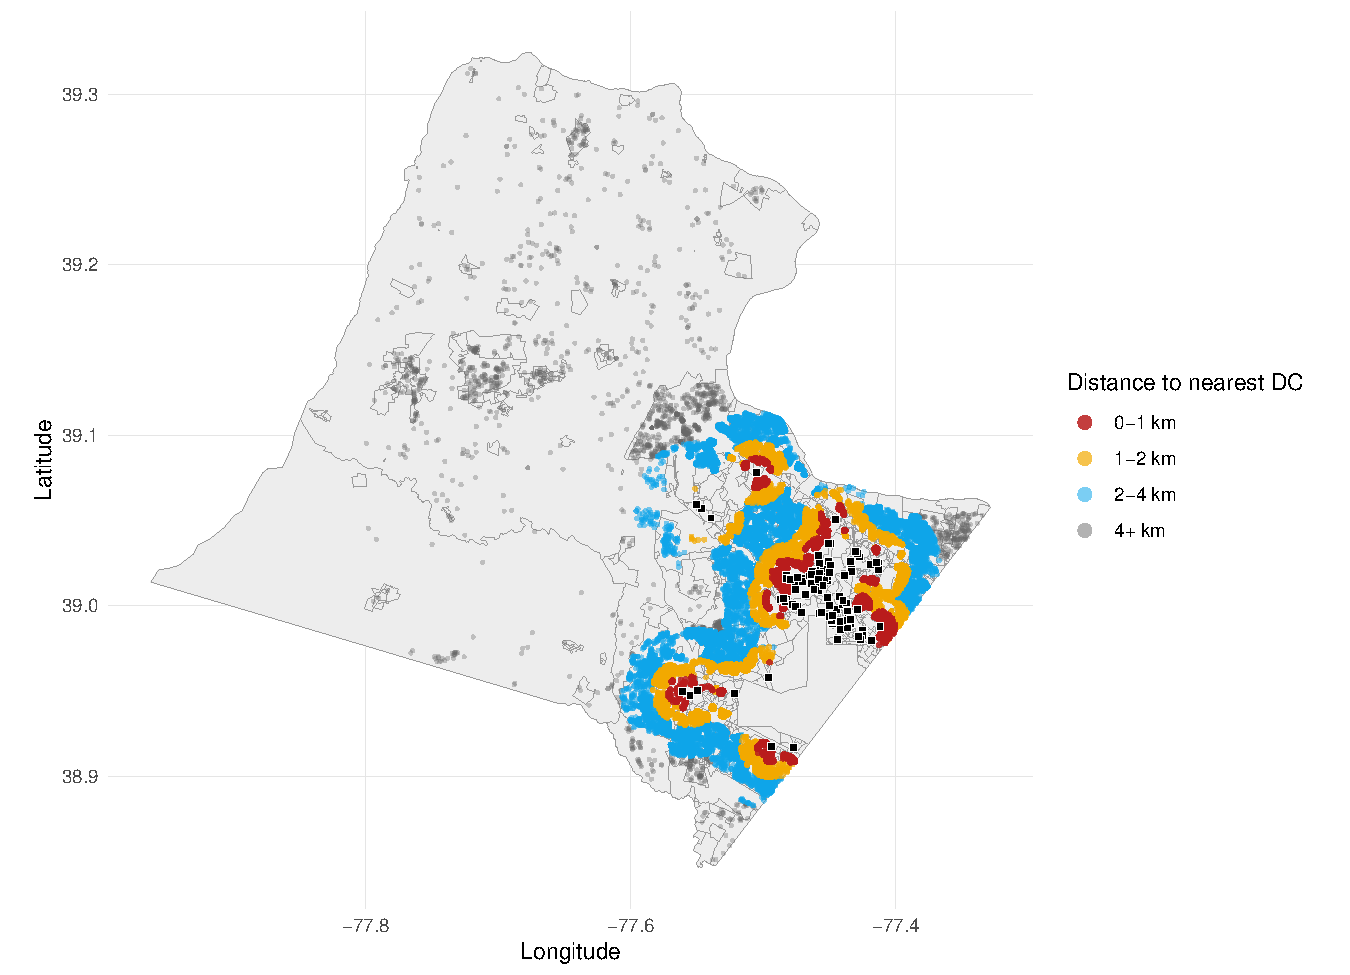
\includegraphics[width=0.95\textwidth]{../Figures/fig_map.pdf}
\caption[Geographic Distribution of Data Centers and Residential Transactions]{Geographic Distribution of Data Centers and Residential Transactions. Black squares are data center facilities, and colored points are residential transactions, 2020--2025, classified by distance to the nearest data center: red $=$ 0--1~km, gold $=$ 1--2~km, blue $=$ 2--4~km, gray $=$ 4+~km.}
\label{fig:map}
\end{figure}

% ==========================================================================
\section{Empirical Strategy}
\label{sec:strategy}
% ==========================================================================

Following \citet{Rosen1974}, I model log sale prices as a function of structural characteristics, location, proximity to data centers, and treatment timing:

\begin{equation}
\label{eq:hedonic}
\log(p_{it}) = \sum_{r} \beta_r \cdot \mathbf{1}[\text{Ring}_{ir}] \cdot \text{Post}_{it} + \mathbf{X}_{it}'\boldsymbol{\gamma} + \alpha_j + \tau_t + \varepsilon_{it}
\end{equation}

\noindent where $\text{Post}_{it} = \mathbf{1}[\text{sale year} \geq \text{permit year of nearest DC}]$, $\mathbf{X}_{it}$ includes living area, bedrooms, bathrooms, age, age squared, construction grade, and property type, $\alpha_j$ is a census tract fixed effect (74 tracts), $\tau_t$ is a year-quarter fixed effect, and the reference category is properties beyond 4 km from any data center. Standard errors are clustered at the census tract level.

To address concerns about heterogeneous treatment effects in staggered settings \citep{GoodmanBacon2021, Roth2023}, I estimate the \citet{SunAbraham2021} interaction-weighted estimator as the primary specification. This defines cohorts by the permit year of each property's nearest data center and estimates cohort-specific treatment effects that are then aggregated into a single ATT. Never-treated properties (beyond 4 km) serve as the comparison group. The Sun-Abraham estimator is robust to heterogeneous treatment effects across cohorts and does not suffer from the negative-weighting problems of standard TWFE.

I estimate event study specifications indexed by years relative to the nearest data center's permit date, with $k = -1$ as the reference category and a window of $[-4, +4]$. Pre-treatment coefficients test the parallel trends assumption. Post-treatment coefficients trace the dynamic path of any disamenity capitalization.

A distinctive feature of data center development is that it is highly visible before completion. Permit applications, site grading, and construction of large industrial buildings generate observable signals over a 12- to 24-month period. If housing markets capitalize expected disamenities at permit issuance or construction start rather than at facility opening, then an event study centered on opening year will underestimate the true effect and may generate spurious "pre-trends'' that actually reflect post-knowledge adjustment. Using permit date as the treatment date narrows timing error relative to opening year but does not eliminate anticipation. For projects like data centers, information likely arrives before permit issuance through zoning applications, site assembly, grading activity, transmission line controversy, and construction visibility. This design reduces the risk that treatment timing is misspecified.

The primary threat is spatial sorting. If lower-quality homes systematically locate near industrial zones where data centers are built, the estimated effect captures pre-existing level differences rather than causal impacts. Census tract fixed effects address time invariant spatial sorting. The repeat sales specification with parcel fixed effects absorbs all time invariant property heterogeneity, though it relies on a smaller and potentially selected subsample.

A second concern is control group contamination. Properties beyond 4 km serve as never treated comparisons, but they may still be affected by data center development through transmission infrastructure, traffic patterns, and county wide fiscal changes. To the extent that control properties benefit from the tax savings funded by data center revenue, the treatment-control contrast understates the true net effect of proximity. This contamination likely attenuates point estimates toward zero, but it also means the "never-treated'' label is an approximation rather than a strict condition.

A notable feature of the results is that the 0--1~km ring is imprecisely estimated while the 1--2~km ring yields the strongest effects. For a genuine localized disamenity, one would expect the closest ring to show the largest effect with monotonic spatial decay. Three factors may explain this anomaly. First, only 2,455 resale transactions occurred within 1~km, limiting statistical power. Second, data centers in Loudoun are overwhelmingly located in industrial and planned development zones, where commercial and industrial parcels typically buffer the nearest residential properties, attenuating close range residential effects. Third, at very close distances, small geocoding errors in parcel centroids produce larger proportional distance errors. This pattern raises questions about the ring based estimates that should temper confidence in their causal interpretation.


% ==========================================================================
\section{Results}
\label{sec:results}
% ==========================================================================

Figure~\ref{fig:price_trends} plots median resale prices by year and distance ring. Properties beyond 4 km command the highest median prices throughout the panel. The trends are approximately parallel across rings, though the persistent level difference reflects spatial sorting.

\begin{figure}[H]
\centering
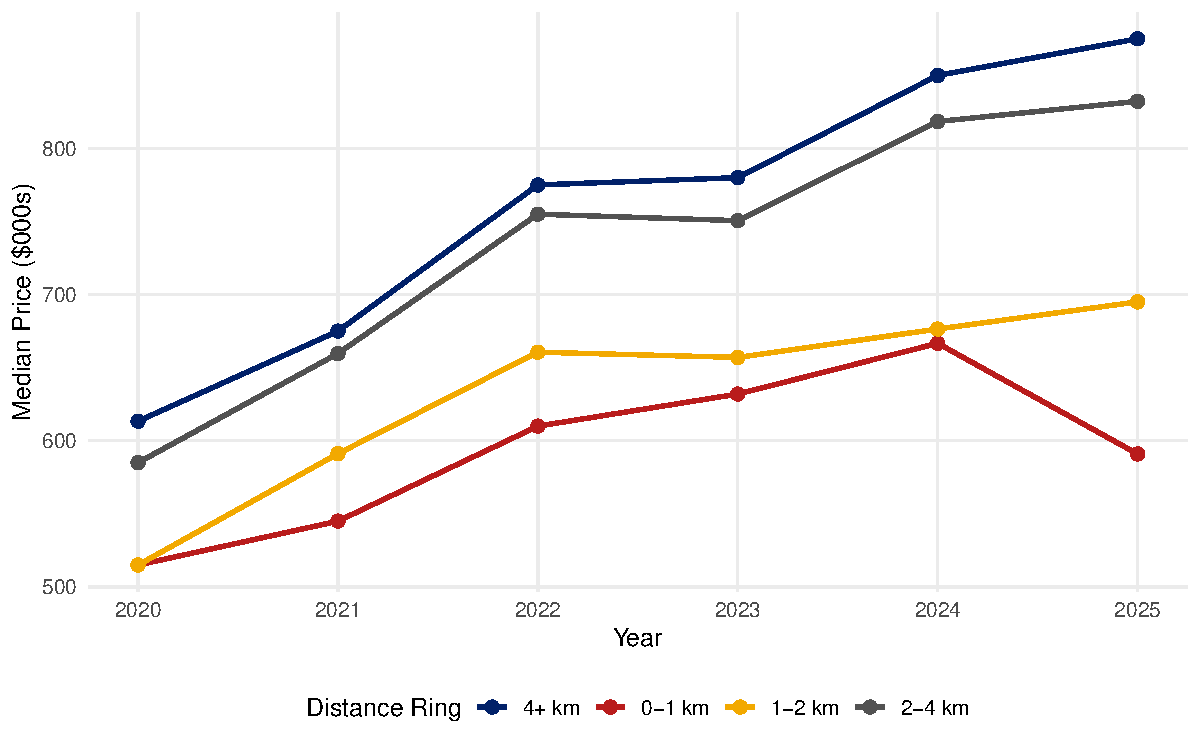
\includegraphics[width=0.85\textwidth]{../Figures/fig_price_trends.pdf}
\caption{Median Sale Price by Distance to Nearest Data Center}
\label{fig:price_trends}
\end{figure}

Figure~\ref{fig:sa} plots the cohort-robust event study coefficients using permit year treatment timing. Pre-treatment coefficients at event times $-3$ and $-2$ are small and not individually significant, but a joint Wald test on these two leads rejects parallel pre-trends at the 5~percent level (TWFE $F(2,49)=3.23$, $p=0.048$; SA $F(2,50)=3.81$, $p=0.029$). Event time $-4$ is excluded from the test because only two observations fall in that bin, both from the sparse 2024 cohort observed in 2020, and its coefficient ($-0.062$, SE $0.008$) is a numerical artifact of bin sparsity rather than evidence of a pre-trend. The test does not reject at the 1~percent level, and the two leads point in opposite directions ($-0.019$ and $+0.019$), which reads more like noise than a systematic pre-trend. The rejection at 5~percent is still a limitation of the design and should temper confidence in the post-treatment estimates. The aggregate ATT is $-0.0134$ (SE $= 0.0048$, $p = 0.008$). At the median assessed value of \$738,730, this implies a price difference of about \$9,600, a statistically significant but economically modest effect.

\begin{figure}[H]
\centering
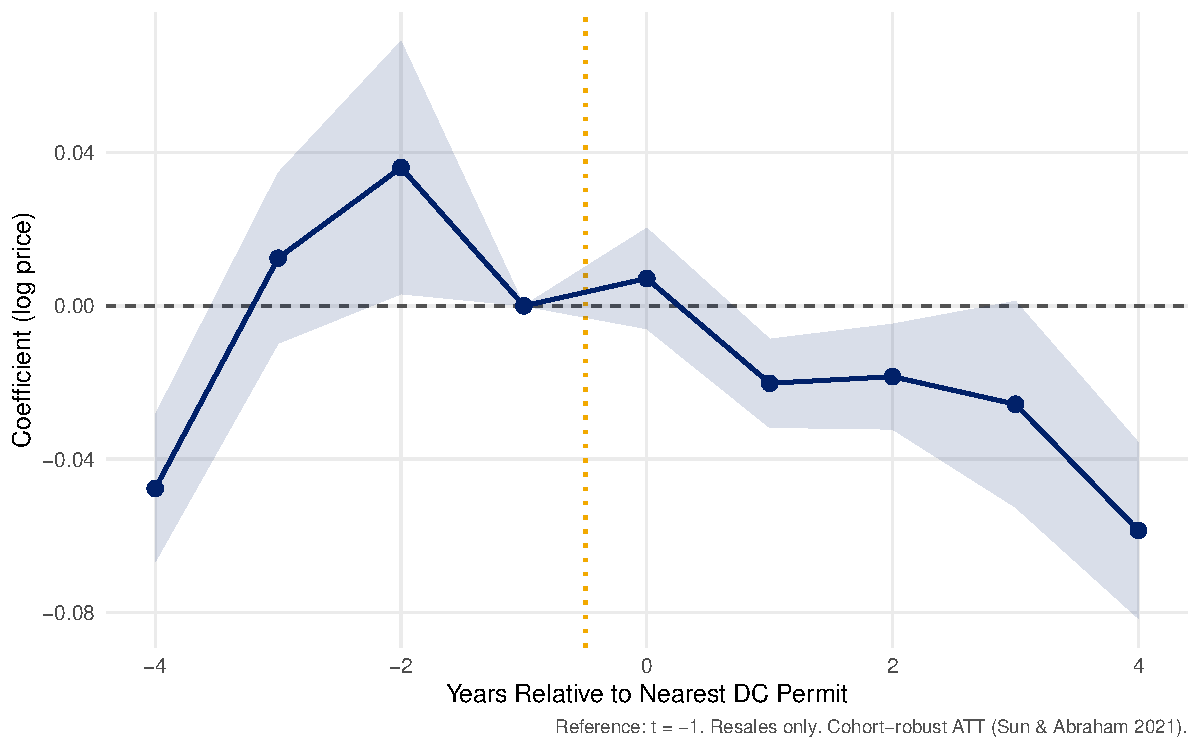
\includegraphics[width=0.85\textwidth]{../Figures/fig_event_study_sa.pdf}
\caption{Sun-Abraham Event Study: Permit Date Treatment (Resales Only)}
\label{fig:sa}
\end{figure}

The magnitude is small compared to power plants ($-3$ to $-7$ percent, \citealp{Davis2011}) or toxic facilities ($-11$ percent, \citealp{Currie2015}), and comparable to the null or small effects found for wind farms \citep{Hoen2015}. This fits data centers being a relatively contained disamenity (noise and visual impacts without air or water pollution). The post-treatment dynamic path is not cleanly monotonic (which one would expect from a disamenity that capitalizes into prices over time), which further weakens the causal interpretation.

Table~\ref{tab:main} presents the full regression results using permit date treatment timing on the resale only sample. Ring$\times$post coefficients are negative across all specifications. The 1--2~km ring is the most precisely estimated, with $p=0.005$ under tract fixed effects (Column 1) and $p<0.001$ under repeat-sales parcel fixed effects (Column 4). The 2--4~km ring is significant in both specifications, while the 0--1~km ring is imprecise, reflecting the thin sample and buffering effects discussed in Section~\ref{sec:strategy}. At the median assessed value of \$738,730, the 1--2~km effect implies a one-time price difference of roughly \$23,000.

\begin{table}[!t]
\centering
\caption{The Effect of Data Center Proximity on Residential Property Values}
\label{tab:main}
\small
\begin{tabular}{lcccc}
\toprule
 & (1) & (2) & (3) & (4) \\
 & TWFE Rings & Cum.\ Exp.\ (sqft) & Cum.\ Exp.\ (count) & Repeat Sales \\
 & Tract FE & Tract FE & Tract FE & Parcel FE \\
\midrule
Ring: 0--1 km $\times$ Post & -0.0236 & & & -0.0144 \\
 & (0.0152) & & & (0.0204) \\
[2pt]
Ring: 1--2 km $\times$ Post & -0.0307$^{***}$ & & & -0.0331$^{***}$ \\
 & (0.0105) & & & (0.0087) \\
[2pt]
Ring: 2--4 km $\times$ Post & -0.0163$^{***}$ & & & -0.0209$^{**}$ \\
 & (0.0051) & & & (0.0101) \\
[2pt]
DC sq ft within 2 km (M) & & 0.0013 & & \\
 & & (0.0040) & & \\
[2pt]
DC count within 2 km & & & -0.0006 & \\
 & & & (0.0014) & \\
\midrule
Structural Controls & Yes & Yes & Yes & No \\
Census Tract FE & Yes & Yes & Yes & --- \\
Parcel FE & No & No & No & Yes \\
Year-Quarter FE & Yes & Yes & Yes & Yes \\
\midrule
Observations & 18,397 & 31,333 & 31,333 & 3,390 \\
R$^2$ (within) & 0.815 & 0.836 & 0.836 & 0.018 \\
\bottomrule
\end{tabular}
\end{table}


Columns (2) and (3) report the continuous cumulative exposure specifications at a 2~km radius. Both the square-footage measure (total data center square footage within 2~km) and the count-based measure (number of data centers within 2~km) yield null estimates. At this radius, the cumulative exposure specification does not recover the effect the ring-based estimates suggest.

Extending the cumulative exposure radius to 4~km produces modestly negative coefficients that are statistically distinguishable from zero (Appendix Table~\ref{tab:appx_cumul_4km}). At the median non-zero 4~km exposure of roughly 3 million square feet, the sqft coefficient implies roughly a 1.3~percent price difference, in line with the SA ATT and with the 1--2~km and 2--4~km ring estimates. The 2~km cumulative null therefore does not represent a robust zero. It reflects that at a 2~km radius, cross-sectional variation in cumulative exposure is largely absorbed by tract fixed effects in Loudoun's clustered data center geography. Expanding to 4~km reintroduces within-tract variation that the fixed effects do not fully absorb, and the effect reappears.

The cumulative exposure results line up with the ring-based estimates rather than contradicting them, but the radius sensitivity is a useful reminder that even the cumulative specification does not yield a tight identification of a causal proximity effect. The repeat sales parcel fixed effects specification (Column 4 of Table~\ref{tab:main}) controls for all time-invariant property characteristics but relies on the subsample of parcels that sold at least twice during 2020--2025. Repeat-sale properties are somewhat selected toward lower-priced, more frequently transacted parcels (Appendix Table~\ref{tab:balance}), so the repeat-sales estimates are best read as local effects for this subsample rather than as estimates for the typical Loudoun homeowner.

Several additional checks assess the stability of the results. A leave-one-tract-out jackknife finds no influential tracts, with the ATT ranging from $-0.0155$ to $-0.0119$ across 51 iterations. A placebo permutation test shuffling treatment dates 500 times places the actual ATT at the 33rd percentile of the placebo distribution ($p = 0.334$; Appendix Figure~\ref{fig:appx_placebo}), a result not distinguishable from randomly assigned treatment timing. A \citet{CallawaySantAnna2021} group time ATT yields $-6.0$ percent, more than four times the Sun-Abraham estimate, though with estimation difficulties for the 2024 cohort. Alternative distance cutoffs (Appendix Table~\ref{tab:alt_rings}) show the 1--2~km ring statistically significant at $p = 0.004$, with the 0--0.5~km and 0.5--1~km rings insignificant. Treatment effect heterogeneity is minimal along both facility size (Large DC minus Small DC difference $=0.009$, $p=0.59$) and cohort timing dimensions (Early minus Late difference $=0.018$, $p=0.39$; Appendix Table~\ref{tab:appx_heterogeneity}), providing some support for the TWFE specifications \citep{Roth2023}. Taken together, the point estimate is stable to sample perturbations but not to treatment-timing perturbations or alternative estimation strategies. These checks are the reason the paper's claim about the housing evidence is narrow. The design does not find robust evidence of economically meaningful localized harm.

To clarify the hierarchy of credibility, I regard the cumulative exposure and ring-based specifications as mutually informative rather than as one dominating the other. The cumulative exposure specification does not rely on arbitrary distance cutoffs, exploits continuous time-varying treatment intensity, and better fits Loudoun's clustered data center geography, but it is radius-sensitive, null at 2~km and modestly negative at 4~km. The ring-based specifications are useful for comparison with the existing literature and for illustrating spatial gradients, but their 0--1~km estimate is imprecise and the pattern is not cleanly monotonic. Taken together, the estimates point toward modest negative effects in the 1--4~km range with fragile identification at any single radius.

The order-of-magnitude comparison is the empirical fact most relevant to the policy question. Even the most negative ring estimate at 1--2~km implies a one-time price difference of about \$22,700 for a median home, concentrated in a few thousand households. The diffuse residential tax cut funded by the data center base is on the order of \$2,512 per year for every one of roughly 130,000 county households. Capitalized at any reasonable discount rate, the present value of that flow dwarfs the most pessimistic point estimate of localized harm, even before accounting for the fact that homeowners within 4~km also receive the same fiscal benefit. Whatever the true causal proximity effect lies in the range the data can support, the asymmetry between concentrated harm and diffuse benefit is large, and it runs in the same direction across every specification I estimate.


% ==========================================================================
\section{Distributional Incidence and Political Economy}
\label{sec:discussion}
% ==========================================================================

Data center tax revenue has enabled a residential property tax rate reduction from \$1.145 to \$0.805 per \$100 of assessed value between 2012 and 2025. For the median homeowner (assessed at \$738,730), this implies annual savings of \$2,512 in 2025 relative to the 2012 rate. The NPV of cumulative observed savings over 2012--2025, discounted at 3 percent, is \$12,086.

This should be understood as an upper bound estimate. Loudoun experienced population growth, rising assessments, and commercial development during this period that would likely have permitted some rate reduction even absent data centers. The cross-county comparison nevertheless provides corroborating evidence. Neighboring Fairfax County, which lacks a comparable data center tax base, maintained a rate of \$1.125 in 2025, 40 percent above Loudoun's. Prince William County's rate was \$0.920 and Arlington County's was \$1.033. While these counties differ from Loudoun in population, commercial composition, and budget priorities, the magnitude of the rate gap points to data center revenue as a primary driver of Loudoun's unusually low residential tax burden.

Data-center-driven transmission and distribution costs amount to \$168--\$444 per year per residential customer \citep{JLARC2024}, spread across roughly 2.36 million Dominion residential ratepayers statewide rather than concentrated in Loudoun. Rate design at the state regulator is the only available response, because local zoning cannot reach a statewide ratepayer base.

The institutional mismatch is structural rather than incidental. Dominion's data-center-driven transmission and distribution capex enters its rate base, the State Corporation Commission approves a revenue requirement, and that requirement is allocated across rate classes by the Class Cost of Service Study. Residential customers absorb their load-proportionate share regardless of where they live within Dominion's service territory, and rising PJM capacity prices propagate the load impact further across the regional market. The roughly 2.36 million Dominion residential ratepayers outside Loudoun have no standing in Loudoun's permit process, and Loudoun's roughly 130,000 households pay the same per-kWh rate as the rest of the Commonwealth. The GS-5 minimum demand charge effective January 2027 imposes contract-demand floors on customers above 25 MW and partially internalizes the externality going forward, but it neither unwinds T\&D capex already in the rate base nor governs the IRP-horizon load that drives the bulk of the \$22 billion estimate. The incidence is mildly regressive on top of being geographically diffuse, because residential electricity is a larger budget share at the bottom of the income distribution than at the top \citep{Borenstein2012}, while the offsetting fiscal benefit accrues to homeowners in one of the highest-income counties in the United States.

The hedonic evidence does not support a stable, tightly identified localized disamenity effect. The Sun-Abraham ATT is statistically significant but economically modest, implying a price difference of about \$9,600 at the median assessed value.

The TWFE ring specifications find larger effects at 1--2~km and 2--4~km, but the closest ring (0--1~km) is imprecisely estimated, an anomalous pattern for a genuine localized disamenity. The event study does not show a monotonically increasing post-treatment path. The cumulative exposure specification is null at 2~km and modestly negative at 4~km. Radius sensitivity prevents it from delivering the tight identification its continuous form might otherwise offer.

This evidence does not support a finding of robust, economically meaningful localized harm. The point estimates are in the small-to-modest range and broadly similar across specifications, but no single specification cleanly identifies a causal effect, and the results as a whole are more informative about what the data rules out than about the precise size of any true effect. Table~\ref{tab:incidence} summarizes the distributional incidence across channels. Fiscal benefits flow to all county homeowners, electricity costs flow to a much larger statewide ratepayer base, and property value effects (to the extent they exist) are a one-time capitalized change concentrated among proximate parcels within 4~km. For homeowners beyond 4~km (the control group in the hedonic design), the evidence shows only fiscal benefits and modest statewide electricity costs.

\begin{center}
\begin{table}[htbp]
\centering
\caption{Distributional Incidence of Data Center Development}
\label{tab:incidence}
\small
\begin{tabular}{llccc}
\toprule
Channel & Who Bears It & Amount (\$) & Type & Affected Pop. \\
\midrule
\multicolumn{5}{l}{\textit{Benefits}} \\
Tax savings (upper bound) & Loudoun homeowners & 2,512/yr & Flow & ${\sim}$130,000 hh \\
\midrule
\multicolumn{5}{l}{\textit{Costs}} \\
Electricity (low est.) & Dominion residential & 168/yr & Flow & ${\sim}$2.36M customers \\
Electricity (high est.) & Dominion residential & 444/yr & Flow & ${\sim}$2.36M customers \\
Property value (0--1 km) & Proximate homeowners & 17,410 & Capitalized & ${\sim}$3,236 parcels \\
Property value (1--2 km) & Proximate homeowners & 22,679 & Capitalized & ${\sim}$12,506 parcels \\
\bottomrule
\end{tabular}
\begin{tablenotes}\small
\item \textit{Notes:} Tax savings are an upper-bound estimate assuming the 2012
rate (\$1.145/\$100) would have persisted absent data center revenue.
Electricity costs from JLARC (2024) range.
Property value amounts from ring specifications applied to median assessed value
(\$738,730).
\end{tablenotes}
\end{table}

\end{center}

\label{sec:legal}

The institutional structure decoupled fiscal capture from localized burden \citep{CalabresiMelamed1972}. The county collected BPP revenue from each new facility while noise, visual impacts, and infrastructure strain fell on nearby residents, and grid costs spilled to Dominion's statewide ratepayers. The by-right regime kept the approval decision at the level of the elected Board, the institution accountable for the residential tax rate and therefore aligned with the diffuse majority that captures the fiscal benefit. The 2025 shift to Special Exception subdivides that decision and grants effective veto to whichever group can mobilize most loudly at the parcel level. \citet{Olson1965}'s collective-action asymmetry tracks the observed regime change. The 3,000--12,500 households within 1--2~km of an existing facility face concentrated per-capita stakes and natural organizing mechanisms in neighborhood associations and the transmission line controversy, while the diffuse majority of roughly 130,000 county households receives \$2,512 per year in tax savings that is not naturally attributed to data centers and therefore not naturally defended through political mobilization. Even \citet{Fischel2001}'s homevoter hypothesis points the same way here, because the median Loudoun homeowner is a net fiscal beneficiary whose property value is sustained by the tax base data centers fund, but the silent capitalized benefit is not the kind of stake homeowners turn out to defend.

The empirical evidence in this paper does not rule out small localized harms, but it fits a setting in which the harm is fragile and economically modest while the benefit is large, broadly shared, and directly capitalized into housing wealth. Under those incidence numbers, transferring veto power to the concentrated minority does not correct a welfare distortion. It creates one. The predictable consequence is a slower data-center pipeline, a tighter county budget, and an erosion of the residential rate cut the diffuse majority currently enjoys. In the limit, the institutional shift can make the median Loudoun homeowner, including most homeowners within 4~km of a data center, worse off to spare a concentrated minority from harms the data are unable to reliably detect.

% ==========================================================================
\section{Conclusion}
\label{sec:conclusion}
% ==========================================================================

This paper examines the distributional incidence of data center development in Loudoun County through three channels, and the channels point in the same direction. The fiscal benefits are large, concentrated in a single jurisdiction, and broadly shared. The median Loudoun homeowner saves about \$2,512 per year, the benefit accrues to roughly 130,000 households, and it capitalizes into housing wealth at every distance from a data center, including for homeowners closest to one. The hedonic evidence for localized property value harm is fragile and economically modest, with point estimates broadly similar across specifications but no single specification cleanly identifying a causal effect, and the most pessimistic ring estimate is an order of magnitude smaller than the forward-capitalized fiscal benefit it offsets. Electricity costs are diffuse, statewide, and being addressed through rate design reform rather than local zoning. The asymmetry across channels is the central empirical fact, and it cuts against the welfare case for restricting development.

Two limitations bound how strongly the political economy argument can be made. The 6-year panel (2020--2025) is short for any hedonic design and precludes long-run effect estimation, so the evidence that the localized harm is small is most credible at the horizons the data can actually see. And I do not observe proposed and denied projects, so the political economy argument rests on the incidence pattern rather than on a direct test of whether approval decisions systematically overweighted fiscal benefits relative to local harms. The remaining limitations (single-cross-section structural controls, timing error in permit year, control-group contamination, mechanism non-identification, and an upper-bound tax savings counterfactual) are discussed in the relevant sections of the paper and cut in directions that tend to attenuate rather than amplify the estimated harm. A longer panel, project-level analysis of approval decisions and hearing records, and direct measurement of noise and visual exposure are the natural next steps and would directly address both of the binding limitations.

The broader lesson is that the move from by-right approval to Special Exception is not a procedurally neutral reform. By-right approval kept siting decisions with the institution accountable for the aggregate fiscal outcome. Special Exception relocates them to a venue that aggregates concentrated parcel-level objections and gives a small group of motivated neighbors an effective veto. On the Olsonian logic, the predictable consequence is systematically fewer approvals than the underlying welfare calculus warrants, which in this setting means a smaller tax base, a slower residential rate cut, and a diffuse majority of homeowners made worse off to spare a concentrated minority from harms the data are unable to reliably detect. As data centers proliferate nationally, the central siting question is therefore not whether public hearings improve democratic input. It is whether the institution that holds them is accountable to the population that bears the net incidence of development, or to the subset that organizes most loudly against it.


% ==========================================================================
\newpage
\appendix
\section{Appendix: Robustness Checks}
\label{sec:appendix}
% ==========================================================================

\subsection{Repeat-Sales Sample Selection}
\label{sec:appx_balance}

\begin{table}[htbp]
\centering
\caption{Comparison of Repeat-Sales and Single-Sale Subsamples}
\label{tab:balance}
\small
\begin{tabular}{lcccc}
\toprule
 & \multicolumn{2}{c}{Single-Sale} & \multicolumn{2}{c}{Repeat-Sale} \\
\cmidrule(lr){2-3} \cmidrule(lr){4-5}
 & Mean & SD & Mean & SD \\
\midrule
Sale Price ($) & 759,126 & 367,574 & 729,981 & 397,562 \\
Living Area (sq ft) & 2,642.3 & 1,114.1 & 2,472.8 & 1,110.9 \\
Bedrooms & 3.5 & 0.9 & 3.4 & 0.9 \\
Bathrooms & 2.9 & 1.1 & 2.8 & 1.0 \\
Age (years) & 22.2 & 18.8 & 24.4 & 23.8 \\
Dist. to DC (km) & 6.6 & 6.4 & 7.3 & 6.8 \\
Assessed Value ($) & 856,644 & 399,163 & 812,950 & 433,627 \\
\% New Construction & \multicolumn{2}{c}{0.0\%} & \multicolumn{2}{c}{0.0\%} \\
\% Within 2 km of DC & \multicolumn{2}{c}{16.7\%} & \multicolumn{2}{c}{16.0\%} \\
\midrule
Observations & \multicolumn{2}{c}{15,008} & \multicolumn{2}{c}{3,390} \\
\bottomrule
\end{tabular}
\begin{tablenotes}\small
\item \textit{Notes:} Repeat-sale parcels are those with two or more transactions
during 2020--2025. DiD subsample restricted to resales near DCs permitted 2019+.
\end{tablenotes}
\end{table}


\subsection{Alternative Distance Ring Cutoffs}
\label{sec:appx_alt_rings}

\begin{table}[htbp]
\centering
\caption{Alternative Distance Ring Cutoffs (0.5/1/2/3 km)}
\label{tab:alt_rings}
\small
\begin{tabular}{lccc}
\toprule
Ring & Coefficient & SE & p-value \\
\midrule
0-0.5 km & -0.0199 & 0.0246 & 0.423 \\
0.5-1 km & -0.0227 & 0.0179 & 0.209 \\
1-2 km & -0.0295 & 0.0098 & 0.004 \\
2-3 km & -0.0203 & 0.0093 & 0.034 \\
\bottomrule
\end{tabular}
\begin{tablenotes}\small
\item \textit{Notes:} TWFE DiD with permit-date treatment on resale sample.  Reference category: 3+ km. Controls: structural, tract FE, year-quarter FE.  SE clustered at census tract.
\end{tablenotes}
\end{table}


\subsection{Opening-Year Treatment Timing}
\label{sec:appx_opening}

Appendix Table~\ref{tab:appx_opening} re-estimates the main ring and Sun-Abraham specifications using the opening year of the nearest data center rather than the permit year as the treatment date. Specifications otherwise match Section~\ref{sec:results}. The ring coefficients and the SA ATT under opening-year timing are comparable in sign and magnitude to the permit-year results.

\begin{table}[htbp]
\centering
\caption{Treatment Timing Robustness: Permit Year vs.\ Opening Year}
\label{tab:appx_opening}
\small
\begin{tabular}{lcccc}
\toprule
& \multicolumn{2}{c}{Permit year (main)} & \multicolumn{2}{c}{Opening year} \\
\cmidrule(lr){2-3} \cmidrule(lr){4-5}
Ring & Coef. & SE & Coef. & SE \\
\midrule
0-1 km & -0.0236 & 0.0152 & -0.0368 & 0.0164 \\
1-2 km & -0.0307 & 0.0105 & -0.0420 & 0.0085 \\
2-4 km & -0.0163 & 0.0051 & -0.0207 & 0.0064 \\
\midrule
SA ATT & -0.0134 & 0.0048 & -0.0182 & 0.0058 \\
Observations & \multicolumn{2}{c}{18,397} & \multicolumn{2}{c}{18,432} \\
\bottomrule
\end{tabular}
\begin{tablenotes}\small
\item \textit{Notes:} TWFE DiD with census-tract and year-quarter fixed effects.
Reference category: 4+ km. Controls: living area, bedrooms, bathrooms, age, age squared, construction grade, property type. SE clustered at census tract.
SA ATT row reports the Sun-Abraham cohort-robust ATT under each timing convention.
\end{tablenotes}
\end{table}


\subsection{Cumulative Exposure at 4 km}
\label{sec:appx_cumul_4km}

Appendix Table~\ref{tab:appx_cumul_4km} extends the cumulative exposure measure to a 4~km radius. Specifications otherwise match Section~\ref{sec:results}. At 2~km the sqft and count specifications yield null effects. At 4~km both measures produce modestly negative coefficients that are statistically distinguishable from zero and consistent in sign and magnitude with the 1--2~km and 2--4~km ring estimates. The radius sensitivity indicates that the 2~km cumulative null is not a robust zero.

\begin{table}[htbp]
\centering
\caption{Cumulative Exposure: 2 km vs.\ 4 km Radius}
\label{tab:appx_cumul_4km}
\small
\begin{tabular}{lcccc}
\toprule
& \multicolumn{2}{c}{2 km (main)} & \multicolumn{2}{c}{4 km} \\
\cmidrule(lr){2-3} \cmidrule(lr){4-5}
Measure & Coef. & SE & Coef. & SE \\
\midrule
DC square footage (per million sq ft) & 0.00128 & 0.00396 & -0.00440 & 0.00167 \\
DC count & -0.00058 & 0.00136 & -0.00179 & 0.00074 \\
Observations & \multicolumn{2}{c}{31,333} & \multicolumn{2}{c}{31,333} \\
\bottomrule
\end{tabular}
\begin{tablenotes}\small
\item \textit{Notes:} Continuous cumulative exposure specifications on the resale sample.
Census-tract and year-quarter fixed effects, structural controls, SE clustered at census tract.
Cumulative measures sum exposure across all DCs permitted prior to each sale date within the stated radius.
\end{tablenotes}
\end{table}


\subsection{Treatment-Effect Heterogeneity}
\label{sec:appx_heterogeneity}

Appendix Table~\ref{tab:appx_heterogeneity} reports interaction tests for facility-size heterogeneity and cohort-timing heterogeneity. The post-treatment indicator is interacted with a binary classifier of the nearest data center, where large facilities are defined as total project square footage above 500{,}000 and the early cohort is defined as permit years 2019--2021 (late is 2022+). Specifications otherwise match Section~\ref{sec:results}, restricted to properties within 4~km. Neither difference is statistically significant, supporting the interpretation that treatment effects are broadly homogeneous along these dimensions.

\begin{table}[htbp]
\centering
\caption{Treatment-Effect Heterogeneity: Facility Size and Cohort Timing}
\label{tab:appx_heterogeneity}
\small
\begin{tabular}{lccc}
\toprule
Interaction & Coefficient & SE & p-value \\
\midrule
\multicolumn{4}{l}{\textit{Panel A: Facility size ($>$500K sq ft vs smaller)}} \\
Small DC $\times$ Post & -0.0273 & 0.0242 & 0.268 \\
Large DC $\times$ Post & -0.0185 & 0.0120 & 0.134 \\
Difference (Large -- Small) & 0.0089 & 0.0165 & 0.592 \\
\midrule
\multicolumn{4}{l}{\textit{Panel B: Cohort timing (permit 2019--2021 vs 2022+)}} \\
Late cohort $\times$ Post & -0.0328 & 0.0274 & 0.241 \\
Early cohort $\times$ Post & -0.0151 & 0.0140 & 0.292 \\
Difference (Early -- Late) & 0.0178 & 0.0207 & 0.392 \\
\bottomrule
\end{tabular}
\begin{tablenotes}\small
\item \textit{Notes:} Interacts the post-treatment indicator with a binary classifier of the nearest DC.
Large DC defined as total project square footage above 500{,}000. Early cohort defined as permit year 2019--2021 (late = 2022+). Sample restricted to properties within 4 km. Census-tract and year-quarter fixed effects, structural controls, SE clustered at census tract.
The ``Difference'' rows test whether treatment effects differ by subgroup.
\end{tablenotes}
\end{table}


\subsection{Placebo Permutation Test}
\label{sec:appx_placebo}

Appendix Figure~\ref{fig:appx_placebo} plots the distribution of Sun-Abraham ATTs under 500 permutations that randomly shuffle each data center's permit year across the observed cohort distribution. The actual ATT ($-0.0134$) falls at the 33rd percentile of the placebo distribution, yielding a permutation $p$-value of $0.334$. The estimate is therefore not distinguishable from what would arise under randomly assigned treatment timing, which is the most direct of the robustness checks discussed in Section~\ref{sec:results} and the reason the paper's claim about the housing evidence is narrow.

\begin{figure}[H]
\centering
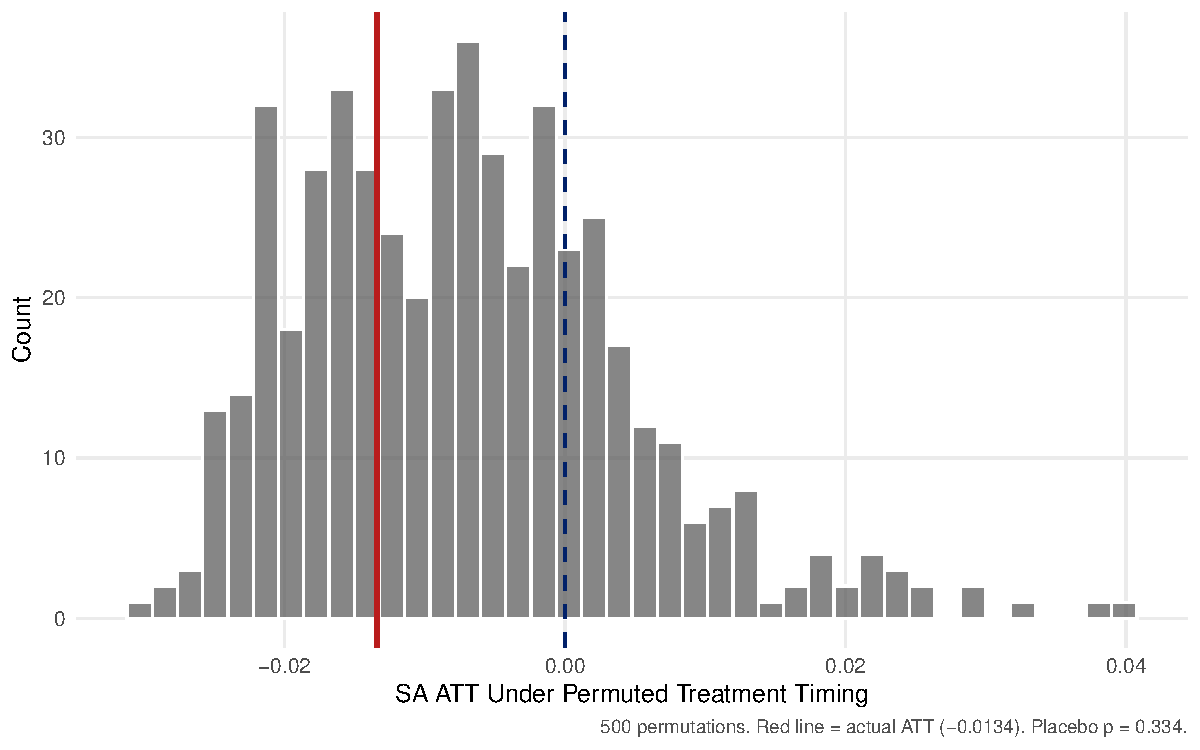
\includegraphics[width=0.85\textwidth]{../Figures/fig_placebo_test.pdf}
\caption{Placebo Permutation Test: Actual ATT vs.\ Shuffled Treatment Dates}
\label{fig:appx_placebo}
\end{figure}

% ==========================================================================
\newpage
\bibliography{references}

\end{document}
